\chapter{Visão Geral}

Para embasar e planejar o projeto a ser desenvolvido, uma proposta de
arquitetura precisa ser feito. Neste capítulo será apresentado tal proposta,
sendo inicialmente explanado a arquitetura esperada por subsistemas, e, ao fim
do capítulo, será mostrada a arquitetura geral do projeto.

\section{Subsistema - Controle e Monitoramento}

O subsistema de controle e monitoramento pode ser dividido em três grandes
componentes: a parte eletrônica da cadeira-de-rodas, um servidor remoto e um
aplicativo que será usado pelos responsáveis de um dado paciente.

A parte eletrônica será composta pelos sensores, que extraírão os sinais do
paciente, os amplificadores e filtros, que farão o tratamento do sinal
extraído, um conversor A/D, responsável por transformação dos dados tratados,
e um sistema embarcado responsável por se comunicar e enviar essas informações
para os outros componentes.

O servidor remoto será um servidor hospedado fora da rede-interna da parte
eletrônica, e poderá ser acessado via \textit{internet}. Se comunicará com
o sistema embarcado da parte eletrônica utilizando comunicação
\textit{via socket}\footnote{\url{https://docs.oracle.com/javase/tutorial/networking/sockets/definition.html}},
apresentará dados ao aplicativo, e o notificará de ocorrência de eventos
críticos.

O aplicativo, que será utilizado pelos responsáveis do paciente, estará
preparado para receber as notificações do servidor e para mostrar os dados em
tempo real.

Abaixo é possível ver o ciclo-de-vida típico do subsistema.

\begin{figure}[H]
  \centering
    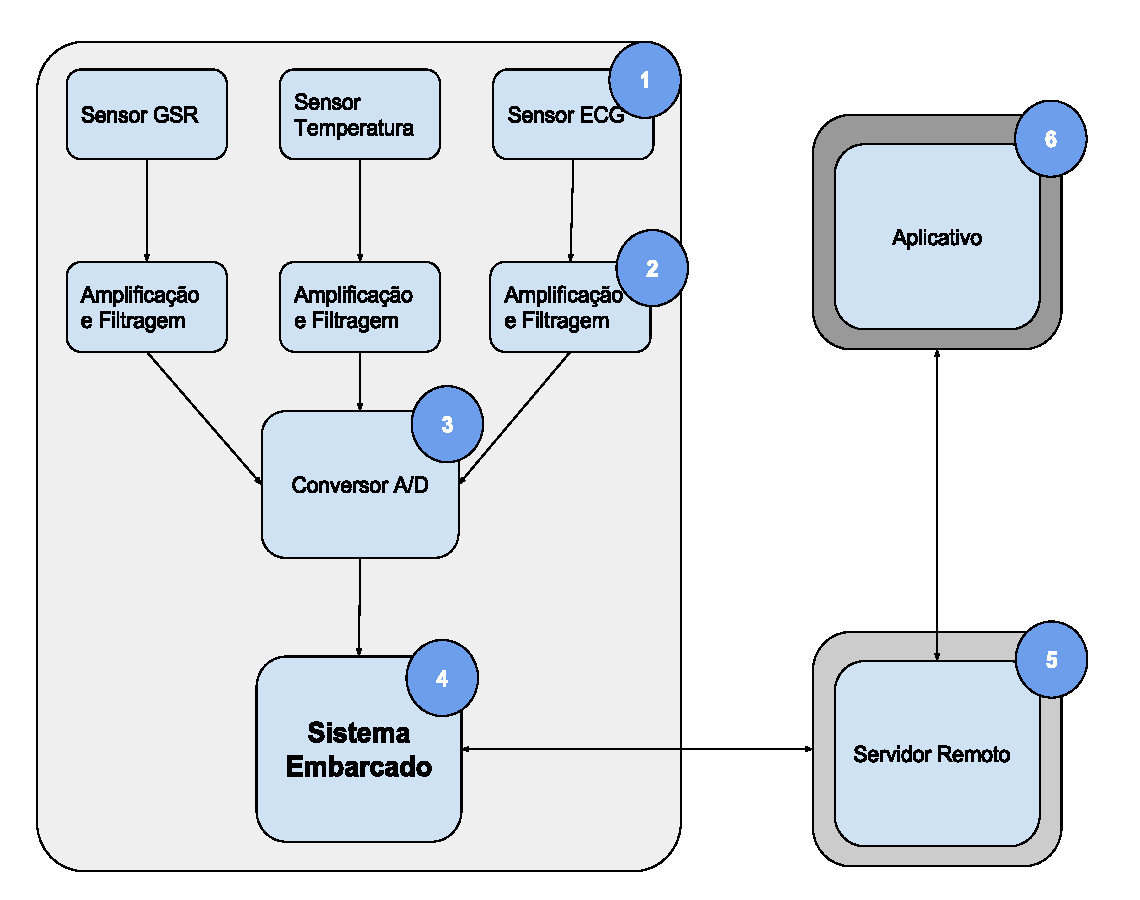
\includegraphics[width=\textwidth]{figuras/arquitetura-monitoramentoecontrole.eps}
  \caption{Fluxo típico do subsistema de Monitoramento e Controle}
  \label{fig:arquitetura-monitoramento-e-controle}
\end{figure}

O passo (1) do subsistema é atuado pelos sensores, que extraírão sinais do paciente;
o passo (2) será atuado pelos amplificadores e filtros, e tratarão o sinal
extraído pelos sensores no passo anterior; no passo (3) os sinais tratados
são convertidos para formato digital, para que possam ser lidos pelo sistema
embarcado; no passo (4) o sistema embarcado recebe as informações do conversor
e abre conexão com o servidor remoto - após, envia as informações recebidas,
quando necessário; no passo (5) o servidor remoto recebe dados do sistema
embarcado e passa informações importantes para o aplicativo, e, por fim,
no passo (6), o aplicativo recebe as informações.

Para o sistema eletrônico de aquisição e condicionamento dos sinais serão 
utilizados eletrodos e sensores. Para os dados de temperatura, será utilizado 
um termistor NTC de 10K, para a captura da frequência cardíaca, será confeccionado 
um sensor para acoplamento ao dedo indicador do usuário. Este sensor funciona 
com um LED que deve estar em contato com a superfície do dedo do usuário, 
e um foto transistor para fazer a captura da luz emitida também em contato 
com o usuário, com isso, é possível capturar dados de frequência cardíaca e oxigenação do sangue.

Além destes, serão utilizados eletrodos para medição de existência galvânica 
da pele (GSR), 
que consistem em dois contatos de prata ou alumínio que deverão estar em contato com a pele do paciente.

Na Figura \ref{sensors} são apresentados modelos comuns dos sensores e eletrodos a serem utilizados.

\begin{figure}[H]
  \centering
    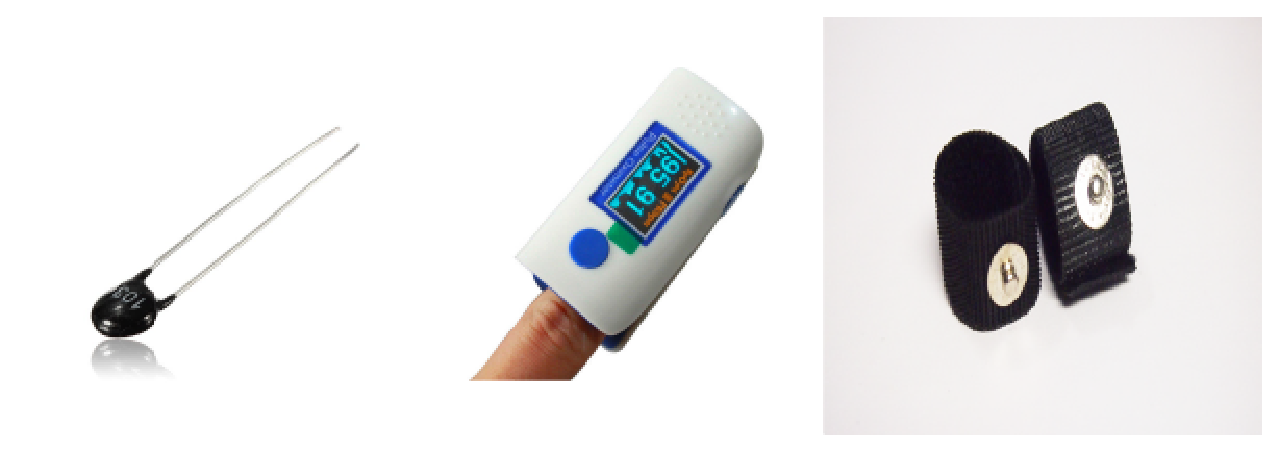
\includegraphics[width=\textwidth]{figuras/sensors.eps}
  \caption{Sensores e eletrodos para captura de sinais: Termistor NTC 10K para temperatura, oximetro de dedo para frequência cardíaca e contatos de prata para captura de GSR.}
  \label{fig:sensors}
\end{figure}

Após a captura destes dados pelos sensores e eletrodos, será implementado 
um sistema de filtragem para o condicionamento dos sinais. Para isso, serão, 
a princípio, utilizadas topologias de filtros \textit{Sallen-Key}, de ordem a ser determinada, 
para a filtragem de frequências interessantes para análise. É importante 
ressaltar que todos os filtros deverão ser projetados e implementados de forma 
ótima para uma melhor captura de dados e para evitar ruídos nas informações apresentadas aos usuários.

\begin{figure}[H]
  \centering
    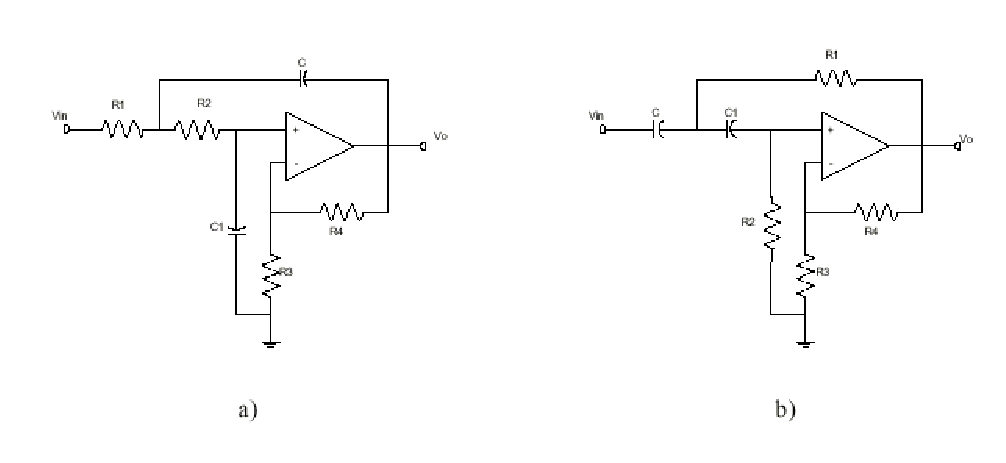
\includegraphics[width=\textwidth]{figuras/sk.eps}
  \caption{Topologias de filtros \textit{Sallen-key}: a) Passa-Baixas e b) Passa-Altas}
  \label{fig:sk}
\end{figure}

Para a incorporação desses filtros, serão utilizados amplificadores operacionais 
TL084 da fabricante \textit{Texas Instruments}. Além do processamento e filtragem 
dos sinais, é necessária uma pré-amplificação que será realizada por amplificadores 
de instrumentações INA118 e INA128, que são amplificadores específicos 
para instrumentação e captura de sinais, fabricados pela \textit{Texas Instruments}.

Importante o ressalte de que todos os sensores e condicionadores utilizados
entregam um sinal analógico, o qual não pode ser processado diretamente
pelo microprocessador selecionado.

A placa de desenvolivmento Raspberry Pi 3, apresentada na Figura \ref{fig:rasp}, 
possui processador de 64-bit Quad-Core ARMv8 de 1.2GHz, 1GB de memória RAM e 
conexões WiFi e Bluetooth, porém, não possui 
entradas para 
conversores A/D (analógico-digital), com isso, torna-se necessário o acoplamento de um conversor externo.

\begin{figure}[H]
  \centering
    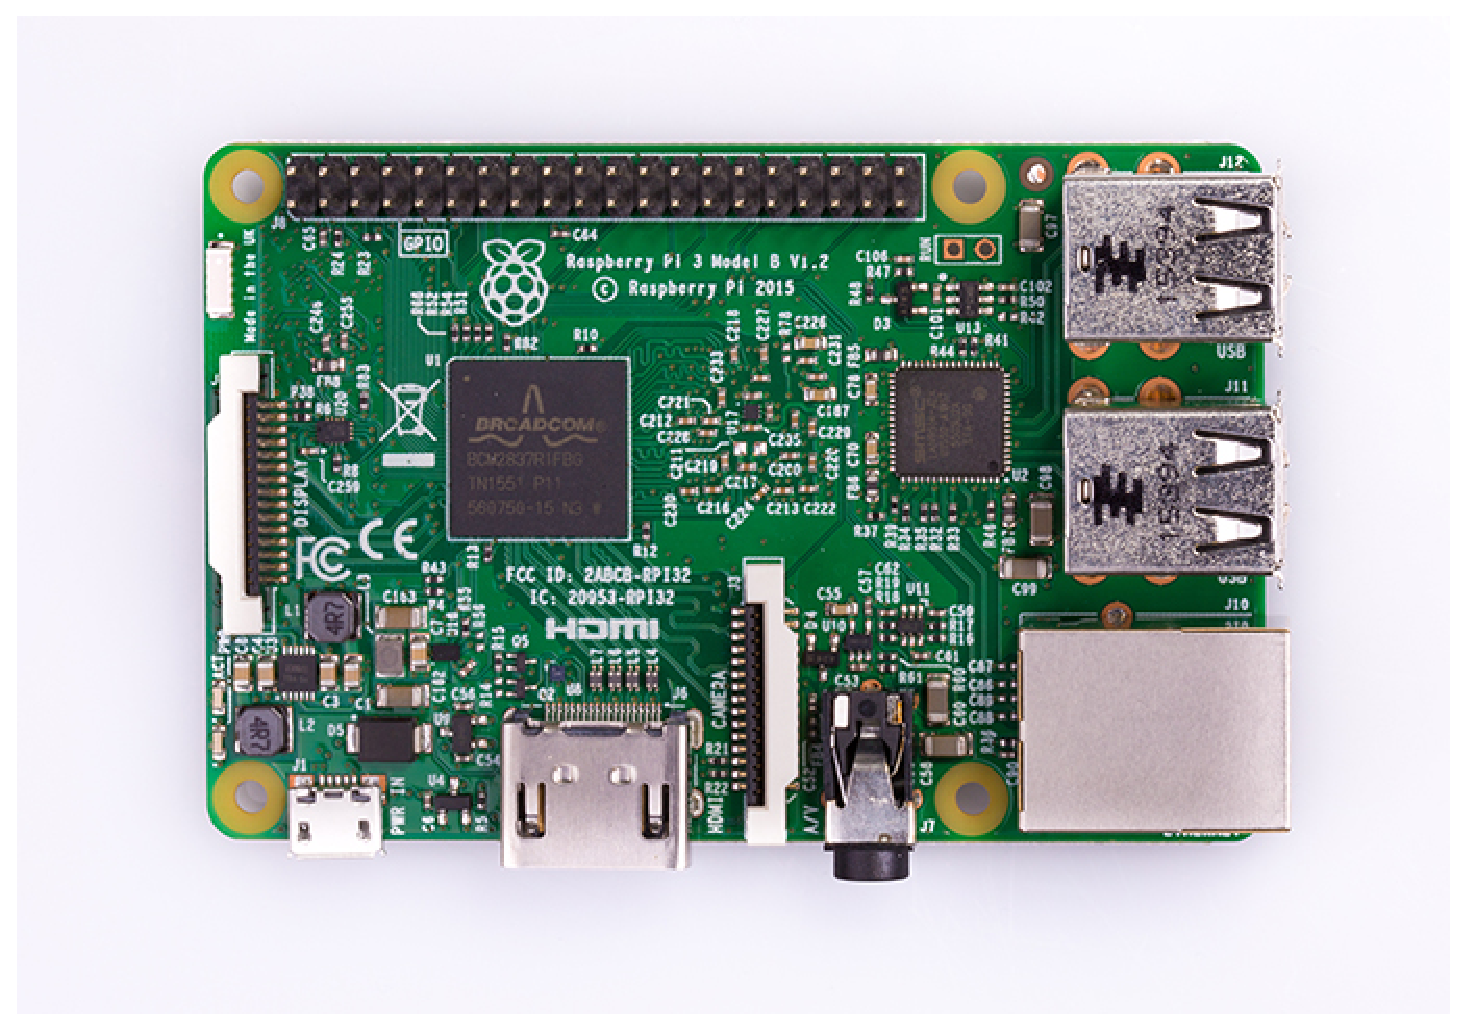
\includegraphics[width=\textwidth]{figuras/rasp.eps}
  \caption{Microcomputador Raspberry Pi 3 Modelo B.}
  \label{fig:rasp}
\end{figure}

Para os fins da aplicação proposta no projeto, foi selecionado o conversor 
ADS1115, mostrado na Figura \ref{ads} que possui 16 bits de resolução e amostragem 
de 800Hz, suficiente para fazer análise de sinais de frequência cardíaca, 
temperatura e GSR, além disso, possui quatro canais de entrada analógica e 
conexão I2C com a Raspberry Pi, diminuindo a quantidade de portas utilizadas no processador. 

\begin{figure}[H]
  \centering
    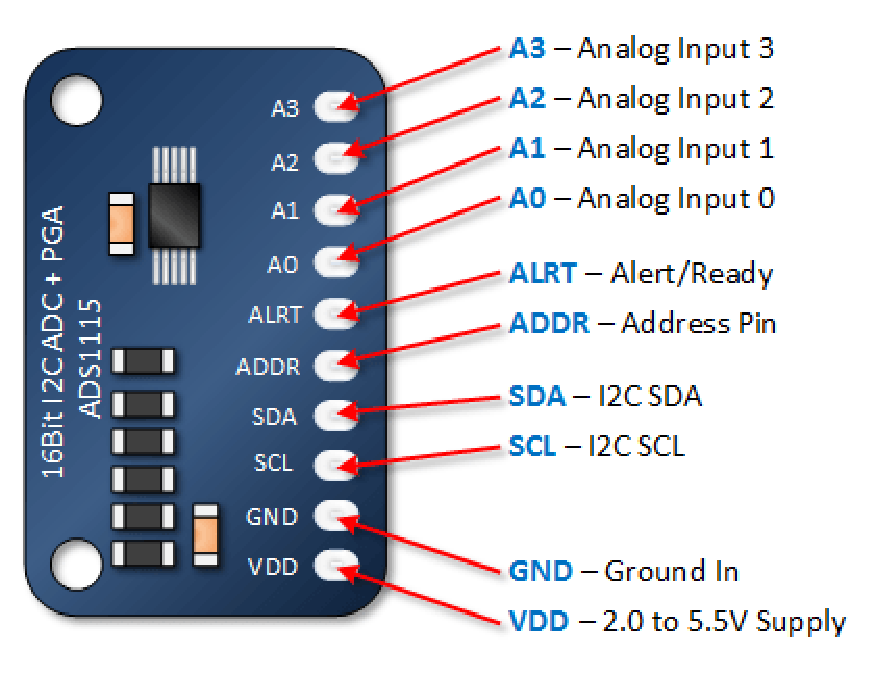
\includegraphics[width=\textwidth]{figuras/ads.eps}
  \caption{Microcomputador Raspberry Pi 3 Modelo B.}
  \label{fig:ads}
\end{figure}



Será implementado, além, um botão de alerta na cadeira de rodas para o envio de alertas 
para os familiares do usuário e um algoritmo programado em linguagem Python para 
detectar picos nos sinais capturados para o envio de dados para o servidor remoto.



\subsection{Tecnologias Utilizadas}

\section{Subsistema - Alimentação}

\section{Subsistema - Estrutura}

\section{Outros}

\subsection{Integração Contínua}
